
\documentclass[man]{apa2}
\usepackage{pslatex}
\usepackage{amssymb}
\usepackage{graphicx}
\usepackage{graphics}
\usepackage{color}
\usepackage{covington}
\usepackage[usenames,dvipsnames]{xcolor}
\usepackage{setspace}
\usepackage[labelsep=none]{caption}

\title{Children's pragmatic inferences as a route for learning about the world}

\twoauthors{Alexandra C. Horowitz}{Michael C. Frank}
\twoaffiliations{Department of Psychology, Stanford University}{Department of Psychology, Stanford University}


\abstract{This study investigated whether children can infer category properties based on how a speaker describes an individual (e.g., saying something is a ``small zib'' implies that zibs are generally bigger than this one). Three- to five-year-olds (N=264) from a university preschool and a children's museum were tested on their ability to make this sort of contrast inference. Four-year-olds made some inferences from adjective choice alone (Experiment 1); performance increased as more cues to contrast were added (Experiments 2 and 3). Control studies show that these findings are not due to the particular properties used or the structure of these tasks (Experiments 4 and 5). These findings suggest that sensitivity to speakers' production choices may help children learn about the world.

~\\

Keywords: pragmatics; language development; adjectives; knowledge transmission}

\shorttitle{Learning through pragmatics}
\rightheader{Learning through pragmatics}

\acknowledgements{Special thanks to the staff and families at the Bing Nursery School and the Children's Discovery Museum of San Jose and to Octavia Zahrt for assistance with Experiment 4. This work supported by a John Merck Scholars Fellowship and ONR grant N00014-13-1-0287. Earlier versions of this work were presented to the Cognitive Science Society in \citeA{horowitz2014}.

~\\

\noindent Address all correspondence to Alexandra C. Horowitz, Stanford University, Department of Psychology, Jordan Hall, 450 Serra Mall (Bldg. 420), Stanford, CA, 94305. Phone: 650-721-9270. E-mail: \texttt{ahorowit@stanford.edu}}

\begin{document}

\maketitle                            


\section{Introduction}

Children learn much important information through explicit instruction (e.g., ``put the fork on the left of the plate'') and generic statements (``forks go on the left''), but not all information is stated directly. Sometimes information is implicit in the particular production choices a speaker makes. For example, if a parent says, ``that's a salad fork,'' she is implicitly conveying that forks vary in the foods they are intended for (and perhaps that most other forks are likely used for non-salad items). More generally, the way we describe the world can reveal to a perceptive observer all sorts of biases about what we find notable, interesting, or worthy of comment---and such biases in turn reflect our views of how the world is structured. Are children able to use these implicit signals for learning? 

We address this question using a simple case study: learning to generalize novel words via minimal contrastive descriptions.  We focus on contrastive word choices, as in the above ``salad fork'' example. Contrastive word choices---the way we use modifiers---can help identify the speaker's intended referent in the current context (selecting the desired fork) but can also jointly signal generalizable knowledge (forks are associated with meal courses). In the current study, we investigate the idea that adults and children may learn generalizable knowledge via inferences about why speakers choose a particular word to convey a message. Because such inferences are subtle and rely on the presumption that a particular modifier is contrastive rather than descriptive, we also examine the ways that other cues support such inferences.

To motivate this case study, we begin by discussing two bodies of research: first, work on children's ability to learn about the world from explicit statements, and second, work on their ability to reason about the implicit knowledge and beliefs underlying other agents' actions (both non-linguistic and linguistic). 

\subsection{Learning from others' explicit statements}

Although learning from the world directly is a very powerful method for acquiring knowledge \cite{gopnik2012b}, there is no way that even the most precocious child-scientist could reconstruct an adult's knowledge from direct experience alone \cite{shafto2012,harris2012}. Instead, children's knowledge comes from a mixture of direct experiences and knowledge transmitted by others. 

Language is one important information source. From the time children begin to speak, they understand that language is used to communicate information \cite{vouloumanos2012}. They expect speakers of the same language to use conventional names for conventional meanings \cite{clark1987, diesendruck2005}, but learn to recognize that individual knowledge such as facts about objects may not be shared \cite{diesendruck2001}. And they also show early knowledge that language can share information that goes beyond the here-and-now \cite{ganea2007}. This early, foundational set of assumptions---that speakers use language in consistent and communicative ways to convey (relatively) abstract knowledge---is critical in allowing children to use language to learn about the world. 

While some language describes the current state of the world (e.g., ``the salad fork is on the outside''), other statements provide more general information that applies across situations (``salad forks go on the outside''). Generic language---cued in a number of ways, including the use of a bare plural (e.g. ``salad forks'')---is a particularly powerful method for conveying such information \cite{leslie2008}. Children can use generic language to infer general properties quite early \cite{gelman2003}. They draw different conclusions from generic statements than non-generic statements, and are more likely to believe that information stated generically is conceptually central and more widely-known \cite{cimpian2009, cimpian2012}. And in some contexts, generic language is not even necessary: The simple use of a label or even the use of particular communicative cues---child-directed speech, direct gaze, or pointing---may signal that a speaker is presenting information that is relevant to a kind, category, or practice \cite{csibra2009, butler2012}. 

Language is such a powerful source of information that preschoolers find it very difficult \emph{not} to believe what they are told.  Three-year-olds can discount inconsistent evidence conveyed through physical markers, but they have a much harder time discounting verbal evidence from an unreliable speaker \cite{jaswal2010}.  When given the option to choose between two potential informants, however, preschoolers can recognize which speaker is more accurate and prefer to trust that speaker \cite{pasquini2007}, retaining this preference even after a time delay \cite{corriveau2009}.  In sum, children favor more reliable speakers when a choice is available, but they display a general bias to trust verbal information.

\subsection{Learning from the knowledge implicit in others' actions}

In nearly all of the work reviewed above, a parent, teacher, or experimenter presents the relevant information explicitly, via a demonstration or explicit utterance. But a parallel line of work suggests that children and even infants are able to make inferences about the \emph{implicit} sources of both linguistic and non-linguistic actions. This literature is critical for motivating our hypothesis here: that such inferences might not just inform guesses about particular agents' knowledge, preferences, or desires, but that they might also be a source of information about the world. 

By their first birthday, babies appear to make inferences about the unseen goals that underlie actions, even in very stripped-down displays \cite{gergely1995}. More generally, infants expect agents to act rationally to achieve their goals in the most efficient way \cite{csibra1998, gergely2003}. In other words, very young children appear sensitive not only to agents' particular actions, but also to the presumed purpose for these actions. Young children also seem to be able to integrate information about constraints into their inferences about goals. For example, infants can distinguish between actions that are produced intentionally versus randomly \cite{xu2009}.  They can also reevaluate the likelihood of particular evidence when physical constraints make it more difficult for certain items to be selected \cite{denison2010b}.  They can even infer that an agent demonstrates a preference by observing a pattern of choices that would be unlikely to occur by random selection \cite{kushnir2010}. 

Critical for our hypothesis here, some evidence suggests that young children can also work backwards from agents' actions to infer generalizable knowledge about objects. \citeA{gweon2010} showed fifteen-month-olds a scenario where an experimenter pulled a series of blue balls from a box and squeezed each toy to produce a squeaking sound. Babies were then handed a slightly different, yellow ball, and their generalizations about whether the new ball should also squeak were measured by their attempts to squeeze the toy. Depending on the evidence they saw, babies made different generalizations: If the blue balls were sampled by the experimenter from a box of mostly blue balls (implying that they were sampled randomly), they were more likely to think that a yellow ball would also squeak. But if they saw the blue balls picked out from a box of mostly yellow balls (intentionally selected for the demonstration of squeaking), they thought the yellow balls were less likely to squeak. In other words, children in this second condition made a general inference about the world (yellow balls don't squeak) based on a surprising thing that someone \emph{didn't} do (not picking out the more common yellow balls). 

Similar to the patterns of reasoning described above, listeners make pragmatic inferences in language comprehension by reasoning about the generating causes of a speaker's (linguistic) action and about the constraints on that action \cite{shafto2012}. Grice's \citeyear{grice1975} maxims of cooperative communication---be truthful, informative, relevant, and clear---provide a framework for inferring meaning from linguistic evidence. If listeners assume that speakers follow these maxims, they can make inferences about meaning that go beyond literal semantics. A number of other theories have also attempted to describe the interplay between intention and production, all preserving the basic idea of pragmatic inference as action understanding \cite{horn1984,clark1996,levinson2000}. 

Just as babies form expectations about sampling likelihoods and infer that violations are intentional and informative (e.g., indicating others' preference or pedagogical demonstrations), children may learn to do the same for language, and make inferences about implicit, intended meaning when speakers' production choices differ from their expectations. While a substantial literature has investigated the specifics of children's pragmatic inference \cite<e.g.>{barner2011,katsos2011}, the general consensus is that children's language learning broadly respects pragmatic principles \cite<see e.g.,>{bloom2002,clark2010,frank2014}.

\subsection{Our current study}

Given that children are able to make sophisticated inferences about the basis for both actions and utterances, we ask whether pragmatic inferences can provide a method for the transmission of information. We investigate preschoolers' ability to infer information about a general class from the specific word choices that a speaker makes in a description. For example, labeling a novel item as a ``tall zib'' conveys not only that this particular item is a tall zib, but also might suggest that height is a relevant property for zibs and perhaps even that other zibs are shorter.   

We focus on adjectives as a case study.  Because adjectives are optional modifiers, they can be included selectively in an utterance to draw contrasts between an intended referent and other unintended alternatives. Three-year-olds can use prenominal adjectives to disambiguate referential targets in their real-time language comprehension \cite{fernald2010}. And four-year-olds are able to infer that adjectives imply contrast (e.g., that ``the red one'' implies a red butterfly rather than red ball when another butterfly is present) \cite{gelman1985}. 

But while previous work has focused on how adjectives are used to identify targets in referential communication tasks, here we examine a novel question. We ask whether adjective use can help listeners infer \emph{what the context is} that would lead a speaker to produce a partiular modified description. We assess the hypothesis that children can infer that a contrastive description conveys not only information about the current referent, but also information about the property of other category members (we refer to these as ``contrast inferences'').  

Adjective contrast inferences have two parts. First, a listener must decide that an adjective is contrastive---meaning that it signals a difference from a set. Not all adjectives are contrastive; for example, in the compliment ``what a nice blue shirt,'' the modifier ``blue''  doesn't typically carry the inference that other shirts are not blue or not nice. Second, given a particular modifier, the listener must infer \emph{what} the implied contrast is: in the example above, that ``tall zib'' implies a contrast in height specifically and perhaps a shorter prototypical zib. In the five experiments below, we tested whether children can identify the appropriate dimension of contrast (the second part of the inference) in contexts that provide a variety of different supports for the identification of contrast (the first part). 

Experiment 1 tested four-year-olds and found that they were able to make some contrast inferences with relatively minimal support. Testing the hypothesis that children's limited knowledge of contrastive adjective pairs accounted for their lower-than-adult performance, Experiment 2 added a pre-exposure to the adjective pairs and found some weak increases in performance. In Experiment 3, in contrast, the stimulus provided strong linguistic cues to contrast, and with this support, even three-year-olds showed evidence of making inferences. Experiment 4 replicated children's performance in the less-supportive contexts from Experiment 1 and ruled out an alternative explanation regarding marked feature dimensions. Finally, in Experiment 5, children succeeded in making contrast inferences in a more open-ended production task, suggesting that they were able to summon to mind the relevant contrast dimension and not just select between visually-presented alternatives. 

\section{Experiment 1}

To investigate preschoolers' inferences about adjective use and category membership, we used a simple triad task.  We introduced children to a novel shape, followed by two similar shapes: one that differed from the first only by size (e.g., tall versus short), and the other that differed from the first only by a different polar feature (e.g., dirty versus clean). We marked the first shape using a prenominal adjective (focused contrastively in its prosody). We then asked children to generalize what they thought other category members usually looked like.  

In discussions of adjective semantics, the size adjectives we used are referred to as \emph{gradable} adjectives because their meaning is relative to the head noun \cite{kennedy2012}---a small sofa is nevertheless bigger than a large mouse. In contrast, our alternative features were \emph{non-gradable}---a sofa or a mouse exposed to water is equally considered wet. For convenience here and below, we refer to this distinction as ``size'' vs. ``feature.'' 

Children could follow at least two plausible strategies in this scenario. First, they could generalize by matching the exact property they heard, reasoning as follows: \emph{You said that this zib was tall, so most zibs are probably also tall}. Second, they could generalize from the property \emph{dimension} they heard, reasoning instead that: \emph{You pointed out that this zib is tall. If most zibs were tall, you probably wouldn't have marked this one's size. So other zibs probably vary by height and can be short.} If children are sensitive to the pragmatic implications of speakers' choices, then they should take the latter route and infer that opting to include an adjective conveys an implied contrast with a set of alternatives, in this case other category members. Note that while in principle the use of a particular adjective only licenses an inference that that property is notable (and thus the category likely \emph{varies} on that dimension), our use of prosody and the question about other exemplars' usual appearance all were intended to bias children to choose the \emph{opposite} to the named property.

\subsection{Methods}

\subsubsection{Participants}

We recruited a planned sample of 48 children from a university preschool into two age groups: 4.0--4.5 years (n=24, mean age 4;4, 12 girls, 12 boys) and 4.5--5.0 years (n=24, mean age 4;8, 15 girls, 9 boys). The preschool is an English language school, and children included in the sample were fluent speakers of English. Two children were excluded for not completing all four trials of the task.

We also recruited a comparison group of 128 adult participants through Amazon's Mechanical Turk (MTurk) online crowd-sourcing service.  Participants all reported being native English speakers and residents of the United States. They were informed that the task was designed for children. Seven participants were excluded for failing to complete the task.  


\subsubsection{Materials}

\begin{figure}[t]
  \begin{center} 
    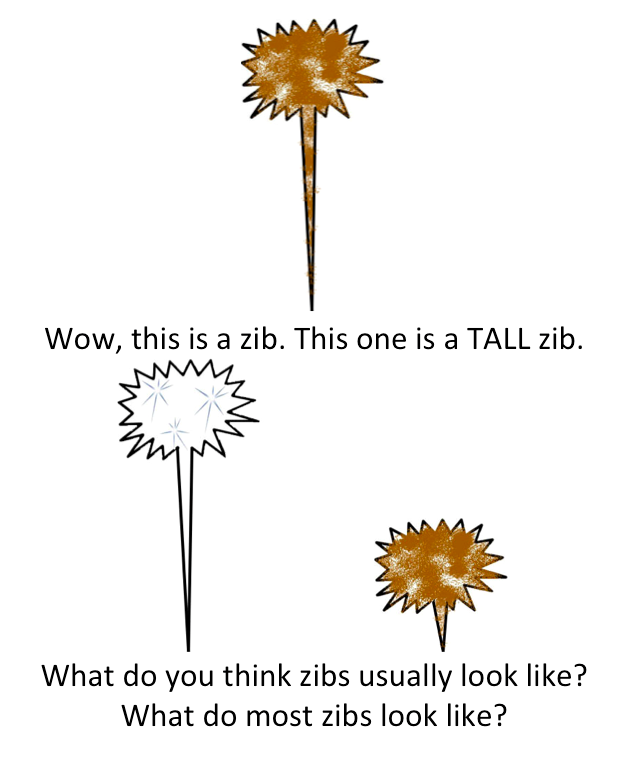
\includegraphics[width=3in]{figures/zib_demo.png} 
    \caption{\label{fig:inanimate_demo} Example test trial. Participants were introduced to an induction example (top) described with either a feature or size adjective. They were then shown two images, one that differed from the induction example by a feature contrast (e.g. dirty versus clean, left) and one that differed by a size contrast (e.g. tall versus short, right), and were asked to point to which picture they thought category members typically look like. In Experiment 3, contrastive framing (``This is a special kind of zib.'') was included before the modified reference. } 
  \end{center} 
\vspace{-10ex}
\end{figure}	

We constructed the experiment as a storybook, illustrated with colorful images. The book contained two training trials and four test trials. Each test trial consisted of a novel shape (induction example) along with a pair of generalization stimuli: one that differed from the induction example only by size (e.g. tall versus short), and one image that differed from the example only by a feature contrast (e.g., dirty versus clean; see example in Figure \ref{fig:inanimate_demo}). Two of the four test trials used size adjectives and two of the trials used feature adjectives. Size terms were \emph{small} (vs. big), \emph{long} (vs. short), \emph{tall} (vs. short), and \emph{short} (vs. long);  feature contrasts were \emph{broken} (vs. unbroken), \emph{pointy} (vs. smooth), \emph{dirty} (vs. clean), and \emph{wet} (vs. dry).  To ensure that children were familiar with the words we used, we included a posttest of two-alternative displays.  Children were able to recognize all of the contrasts used in our task, with 96\% for 4.0--4.5 year-olds and 98\% for 4.5--5.0 year-olds.  

\subsubsection{Procedure}

The experimenter read the storybook with children individually in a quiet room at their preschool. To begin the book, children were introduced to a character named Allen the Alien who was visiting planet Earth.  They then participated in two training trials containing familiar items to teach Allen about some things on Earth and get children used to the study design.  Training trials featured adjectives other than those used in test trials, and training pictures displayed only one relevant contrast choice.  For example, children were shown a picture of chocolate milk followed by two pictures, one of plain milk and one of orange juice. Children were told, ``This is milk. This is \emph{chocolate} milk.  What does milk usually look like?  What does most milk look like?'' and prompted to point to the picture. 

Our training examples were framed around identifying a prototypical case of a noun category in order to help children understand that the goal of our task is to find what members of a category usually look like. Although we expected children to comprehend \emph{most} and \emph{usually} at the ages we tested \cite{halberda2008}, the training trials were intended to  help illustrate this relationship further. On the rare occasion that children answered incorrectly, the experimenter repeated the statements and encouraged children until they answered correctly.  

After the training trials, children participated in four test trials.  For each test trial, children were shown a picture of an induction example and told something about it, e.g. ``This is a zib. This is a tall zib.''  They were then shown two similar pictures, one that differed from the exemplar only by the target feature dimension (e.g., a tall clean zib) and one that differed from the exemplar only by size (e.g., a short dirty zib), and were asked ``What do you think zibs usually look like?  What do you think most zibs look like?'' 

Children were assigned to one of two lists, counterbalanced for adjective type and picture order.  Adjectives (in this and all subsequent studies) were focused using contrastive stress. The experimenter sat next to the child and avoiding gaze cues while children pointed to their selections.  Responses were coded online and double-coded offline using a video recording of the testing session.  The task took about ten minutes to complete. 

The task was adapted to an online format for adult participants. They viewed a single trial composed of one of the picture triads and read the same text that was spoken to children. We used only a single trial for adults to avoid inducing task demands caused by repeating the same type of inference. Picture type, side, and adjective were counterbalanced across participants.  Adults indicated their response using a radio button below their image selection and were paid 25 cents for completing the task, which took about two minutes. 

\subsection{Results and discussion}

\begin{figure}[t] 
  \begin{center} 
    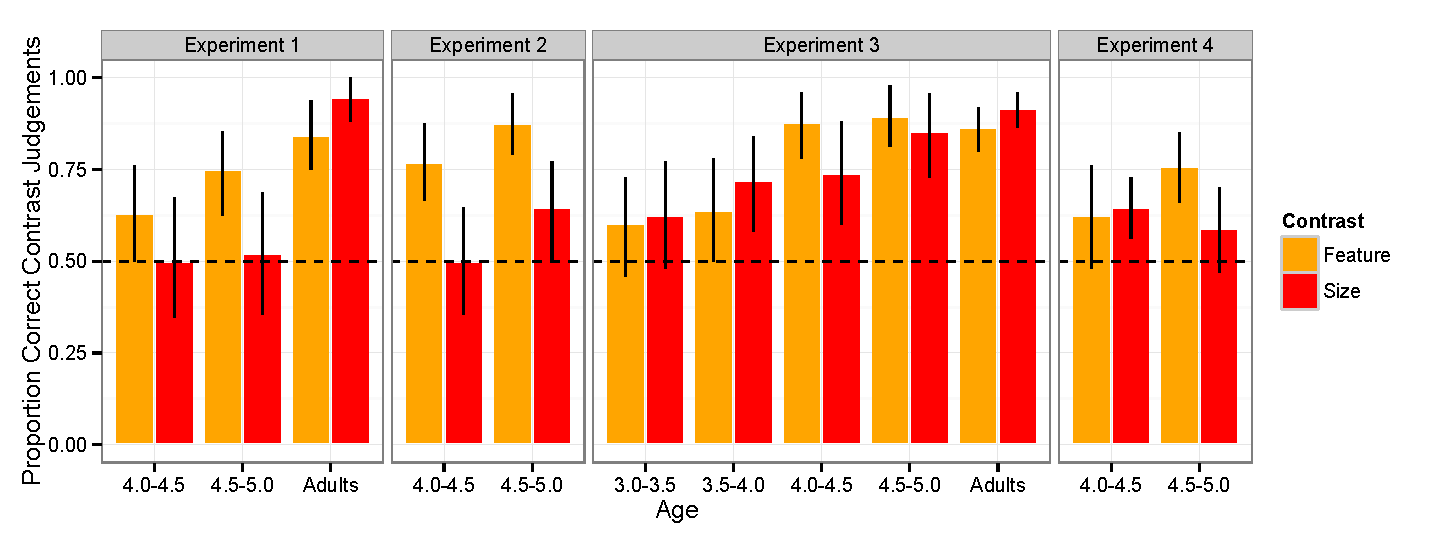
\includegraphics[width=6.5in]{figures/experimentsReorder.pdf} 
    \caption{\label{fig:experiments1thru4} Preschoolers' and adults' mean proportion correct contrast judgements in Experiments 1--4.     
  %  \caption{\label{fig:experiments1thru4} Mean proportion correct contrast judgments for preschoolers and adults in Experiment 3. 
  Yellow bars depict feature adjective trials and red bars depict size adjective trials. Dashed line represents chance; error bars show 95\% confidence intervals computed by non-parametric bootstrap.}
  \end{center} 
  \vspace{-10ex} 
\end{figure}

Inferring a dimension of contrast from a single adjective cue was challenging for children. We categorized a response as correct---representing what we will call a \emph{contrast inference}---if participants selected the item that differed from the exemplar along the referenced dimension (e.g., they chose the short item if the exemplar was referred as ``tall,'' and the clean item if it was described as ``dirty'').  Contrast selections in size trials were especially low, while contrast judgements in feature trials remained higher. Averaging across adjective types, 4.0-year-olds were not above chance ($t(22) = 1.10$, $p = .28$), but 4.5-year-olds were ($t(23)=2.18$, $p = .04$). Raw data and analysis code can be found at REMOVED FOR BLIND REVIEW. 

Breaking performance down by adjective type, on feature trials the younger 4s' performance was marginally significant in a test against chance, while the older 4s' performance was significantly different from chance ($t(22) = 1.82$, $p = .08$ and $t(23)=3.71$, $p = .001$). Both groups' performance did not differ from chance for size adjectives. Overall, the task was difficult but older children could make contrast inferences at above-chance levels for feature adjectives. 

A possible explanation for these findings is that contrast inferences were in fact not warranted by the subtle cue of a single adjective. Ruling out this explanation, adults were near ceiling at making contrast selections for both feature and size terms in this task. These findings indicate that prenominal adjective use is a strong cue to contrast for mature listeners, and children's sensitivity to the implications of these descriptive choices is still developing.

For children, a potential source of the asymmetry between feature and size adjectives could be due to the relatively greater contrast implied by our featural adjectives. Saying that something is ``dirty'' almost always implies a changed state from having been clean at another point in time. In contrast, saying something is ``tall'' can imply that there are shorter others---but it can also simply reflect some sort of general, stable comment on height. If this ambiguity about the contrastiveness of the size adjectives was the source of the low performance in this task, familiarizing children with opposite pairs used in the task might help them better make contrast inferences for these terms at test. In Experiment 2, we included an Alternatives Pre-Exposure book before the task to examine whether it might increase performance for size adjectives by virtue of highlighting the contrastive use of alternative size terms. 

\section{Experiment 2}

Previous work on pragmatic inference has suggested that one major problem for preschool children in making inferences about contrasting terms is summoning to mind alternative word choices that could have been used (e.g. that ``some'' is a weaker alternative to ``all''; \citeNP{barner2011}). For this reason, we attempted to alleviate this burden in our task by providing children with pre-training on the relevant contrasts used at test. In Experiment 2, we reran the same procedure as in Experiment 1 but preceded the task with a storybook highlighting the polar opposite terms. The goal of this pre-exposure was to remind children that, for example, ``short'' is the alternative to ``tall.'' We predicted that the increased experience comparing adjective alternatives in this condition would help support children's ability to make contrast inferences at test.

\subsubsection{Participants}

We recruited a new sample of 48 children from the same university preschool: 4.0--4.5 years (n=24, mean age 4;4, 12 girls, 12 boys) and 4.5--5.0 years (n=24, mean age 4;8, 11 girls, 13 boys). Two children were excluded for not completing all four trials of the task.

\subsubsection{Materials}

Stimuli were identical to Experiment 1. In the pre-exposure phase, participants read a book with clipart images of familiar items depicting the same size and feature contrasts terms portrayed in the test book. Opposites were paired so that scalar contrasts were viewed simultaneously and stated consecutively (e.g. ``Here is a small teddy bear. Here is a big teddy bear.'').  Sample images are presented in Figure \ref{fig:book_demo}.

\begin{figure}[t] 
  \begin{center} 
    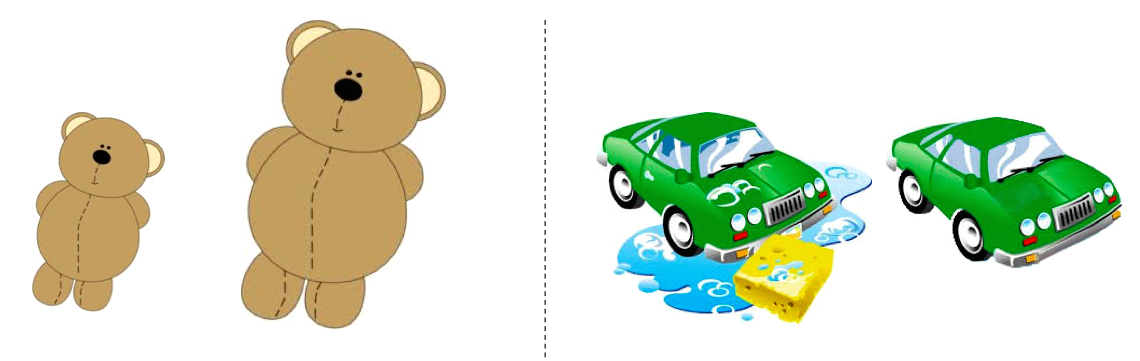
\includegraphics[width=4in]{figures/aliens_book_demo_mod.png} 
    \caption{\label{fig:book_demo} Sample images from the Alternatives Pre-Exposure book in Experiment 2. Left: example size contrast (small bear vs. big bear). Right: example feature contrast (wet car vs. dry car).}
  \end{center} 
\vspace{-10ex}
\end{figure}

\subsubsection{Procedure}

The procedures were identical to Experiment 1 except for the addition of reading the pre-exposure book prior to test. Children were told that they would be reading two books in the experimental session. Before moving on to the test book, the experimenter read the pre-exposure book with children. As in Experiment 1, contrastive prosody was used for all adjectives in the Pre-Exposure book as well as in the test trials.

\subsection{Results and discussion}

Contrast selections were still difficult for children, but---consistent with our hypothesis---the alternatives pre-exposure led to above-chance performance by both age groups. Although the test trials were identical to those in Experiment 1, children in Experiment 2 were above chance ($t(23) = 2.33$, $p = .03$ and $t(23) = 6.33$, $p < .0001$), aggregating across adjective types. Breaking down by adjective types, the younger 4s were above chance for feature but not size adjectives ($t(23) = 4.51$, $p = .0001$ and $t(23)=0$, $p = 1$). Older children were above chance on both ($t(23) = 8.31$, $p < .0001$ and $t(23)= 2.07$, $p = .05$). Nevertheless, no pairwise $t$ tests between the Experiments 1 and 2 were significant, so we interpret these results with caution. 

We next analyzed our results using a logistic mixed model that included all interactions of age, adjective type, and Experiment (1 or 2). This model included random effects of contrast for each participant. Here and below, we followed the guidelines of \citeA{barr2013} with respect to random effect structure: we began with a ``maximal'' model that included random effects of contrast by subject and random effects of contrast by item, but pruned away these effects if the model did not converge (as in this case, where we removed all random effects by item). 

In our first model, with interactions of age, adjective type, and experiment, we found that no effects reached significance. In particular, this model did not increase fit over a model that only included main effects ($\chi^2(4) = 2.47$, $p = .65$), suggesting that it may have been over-parameterized relative to the amount of data we had for the two experiments. A main-effects only model included a significant effect of adjective type such that children made fewer contrast selections on size trials than feature trials ($\beta = -1.08$, $p < .0001$). It also included marginal effects of age and experiment ($\beta = 1.04$, $p = .07$ and $\beta = .50$, $p = .09$, respectively), indicating that older children performed somewhat better than younger children, and that performance was somewhat higher in the Experiment 2 than Experiment 1. 

In sum, the results from Experiment 2 provide further support for the ability of four-year-olds to make contrast inferences. We also saw some signs that pre-exposure to a storybook that used the target adjectives contrastively improved performance, consistent with the idea that increasing the recognition of pragmatic contrasts helped children to make the appropriate generalization. Nevertheless, this effect was small and was at best marginally significant in some analyses. In the next experiment, we investigated an alternative support to contrast inferences: making the fact of contrast extremely salient by highlighting that an exemplar was ``special.''

\section{Experiment 3}

In Experiment 3, we tested contrast inferences in a linguistic context where the fact of contrast was highly salient. We reran the same procedure as in Experiment 1 but in Experiment 3 we marked that each exemplar was ``a special kind of'' category member (e.g., ``This is a \emph{special kind of} zib. This is a tall zib''). If recognizing that an adjective is being used contrastively is the most challenging part of the inference for children, then this manipulation should increase performance. Note however, that even with this supportive framing, children must still perform an inference: they must still recognize that the adjective the speaker uses implies a contrast along that dimension and identify the reversed dimension as the correct match.

\subsection{Methods}

\subsubsection{Participants}

We expanded our age range in this study to include both 3- and 4-year-olds. We recruited a planned sample of 96 children in four age groups: 3.0--3.5 years (n=24, mean age 3;3, 11 girls, 13 boys), 3.5--4.0 years (n=24, mean age 3;9, 8 girls, 16 boys), 4.0--4.5 years (n=24, mean age 4;3, 12 girls, 12 boys), and 4.5--5.0 years (n=24, mean age 4;8, 14 girls, 10 boys).  Approximately half of the sample was recruited from the same university preschool (n=52) and half was recruited from a local children's museum (n=44); recruitment location was roughly even across age groups. Children from the nursery school and the museum were demographically similar in terms of language exposure, ethnic backgrounds, and parental education, as reported by parents from each location. Samples from both locations were mainly composed of educated, Caucasian, middle class families. We tested for effect of location, and found no differences.

At the museum, parents accompanied their children and were asked to fill out a short demographic form about the child's language background. In our partnership with the museum, we invite any interested visitors to participate in our studies rather than prescreening children to meet our language requirements or to counterbalance all demographic factors \cite{callanan2012}. As a pre-specified selection criterion, only children who were reported to hear English at least 75\% of the time were included in the final sample.  Eight participants were excluded from analysis based on this criterion. An additional two participants were excluded due to interruptions from family members during the testing session, and two were excluded for not completing all four experimental trials. 

We also ran a group of 128 adult participants on MTurk.  All participants were reported to be US residents and native English speakers.  They were informed that the task was designed for children. Three were excluded for failing to complete the task. 

\subsubsection{Materials}

Materials were identical to Experiment 1.

\subsubsection{Procedure}

Procedures were identical to Experiment 1, with the only difference that the induction shape was introduced as a ``special kind of'' that category member.

\subsection{Results and discussion}


Preschoolers' ability to make correct contrast inferences increased across the age range we tested (Figure \ref{fig:experiments1thru4}).The youngest children in our sample (age 3.0--3.5 years) were marginally above chance ($t(23) = 1.84$, $p = .08$) in their contrast inferences across adjective types, and all other age groups were above chance (all $p$s $< .01$).

To measure differences across adjective types and age groups, we fit a logistic mixed effect model predicting correct responses as the interaction of age and contrast type, with random intercept and slope (reflecting contrast type) for each participant and a random intercept and slope (again by contrast type) for each item. Children made increasingly more correct contrast judgments with age ($\beta = 1.52$, $p < .0001$). There was no significant effect of contrast type (feature vs. size adjectives), and no interaction between age and contrast type, suggesting that participants across ages did not differ in their responses to different property types.  

We next tested whether the ``special'' manipulation in Experiment 3 led to an increase in performance over Experiment 1. We consolidated the data from both Experiments and fit a single logistic mixed effects model. Models with larger random effects structures and higher order interactions failed to converge, but we fit a model with fixed effects of experiment, contrast, and age, as well as interactions of age by contrast and experiment by contrast (with no three-way interaction). We included random intercepts for each participant. This model showed a significant main effect of experiment ($\beta = 1.31$, $p = .002$) and no interaction between experiment and contrast, confirming a gain in performance due to the ``special'' manipulation. 

These results further support children's ability to perform contrast inferences and indicate that identifying that an adjective is meant contrastively is likely the most challenging part of such inferences, at least for older children. With convergent cues that signaled contrast---the ``special'' framing, prosodic focus, and the structure of a test question that asks what category members are ``usually'' like in the context of a contrasting alternative---older four-year-olds performed at the same numerical level to adults.

\section{Experiment 4} 

Experiments 1 -- 3 show that preschoolers can infer the appropriate dimension of contrast from the presence of an adjective. In these experiments, however, children's performance could have been an artifact of the particular modifier terms we used, which tended to convey marked, atypical properties. For example, children might have heard ``dirty'' and responded that other category members tend to be clean due to a baseline assumption that cleanliness is a more common, default state (rather than due to having made a contrast inference per se). In Experiment 4, we replicated our basic experimental paradigm, but fully counterbalanced adjective references across both ends of the opposite scales. Instead of comparing only one of a pair of feature or size terms---``dirty'' vs. ``tall''---we also included trials containing references to their opposites---``clean'' vs. ``short.''  As a result of this design choice, we also included eight (rather than four) trials per child, increasing our overall statistical power.

\subsection{Methods}

\subsubsection{Participants}

We recruited a new planned sample of 48 children in two age groups: 4.0--4.5 years (n=24, mean age 4;3, 12 girls, 12 boys), and 4.5--5.0 years (n=24, mean age 4;8, 12 girls, 12 boys).  Half of the sample for each age group was recruited from the university preschool and half was recruited from the children's museum.

\subsubsection{Materials}

Stimuli were combined from---and mostly identical to---those used in Experiments 1--3, with some minor modifications. The stimulus set was composed of eight experimental trials.  Each trial depicted a unique, nameable feature opposite pair (\emph{dirty---clean, wet---dry, pointy---round, hot---cold. dark---bright, open---closed, soft---hard,} and \emph{full---empty}). Four size pairs (\emph{big---small, tall---short, fat---skinny, long---short}) were used twice across the test set, with each term represented as an exemplar once per participant.  All items for this experiment are show in Table 1 of Appendix A. 

\subsubsection{Procedure}

The procedure was identical to Experiment 1. Children participated in 8 trials, however, which were counterbalanced by list order, adjective type (feature vs. size), polarity of the opposite term (e.g. ``dirty,'' ``clean,'' ``tall,'' or ``short''), and target location. 

\subsection{Results and discussion}

Overall, performance in Experiment 4 was similar to the Experiment 1 (Figure \ref{fig:experiments1thru4}). If anything, the results were stronger, providing evidence against the argument that feature markedness led to our previous findings. 

Both younger and older 4s were reliably above chance ($t(23) = 3.05$, $p<.01$ and $t(24) = 3.99$, $p<.001$, respectively). Younger 4s made contrast selections reliably above chance in size trials ($t(23)=3.44$, $p<.01$) and marginally above chance for feature trials ($t(23)=1.73$, $p=0.09$). Older 4s showed a slightly different pattern, selecting the contrast reliably on feature trials ($t(24)=5.32$, $p<.0001$) but not performing significantly above chance on size trials ($t(24)=1.56$, $p=.13$). 

We ran a logistic mixed effect model predicting correct responses as an interaction of contrast type and age, with a random intercept and contrast term for both each participant and item.  A marginal effect of adjective type emerged, such that children made more contrast selections for size than feature trials overall ($\beta = 8.59$, $p = .09$). There was also a marginally significant interaction between trial type and age, reflecting higher performance on feature trials with age ($\beta = -2.08$, $p = .07$). 

In our final experiment, we test the extent to which findings in these previous experiments are driven by the use of a two-alternative forced choice paradigm, which highlights contrast by providing alternatives that contrast on individual features.

\section{Experiment 5} 

In Experiment 5, we measured children's contrast inference performance in a free-response task. One possible interpretation of Experiments 1--4 is that children might not be making contrast inferences immediately, but they might recognize that such an inference is required by the two-alternative forced-choice format of the experiment. A free response task circumvents this issue by testing children's interpretation of the concept without asking them to choose between alternatives. For the linguistic framing in this experiment, we chose an intermediate level of support for contrast; more supportive than Experiments 1 and 2, but less extreme than Experiment 3: we told children that there were ``different kinds'' of the target item.

\subsection{Methods}

\subsubsection{Participants}

We recruited a new planned sample of 24 4-year-old children (mean age 4;6, 12 girls, 12 boys) from the local children's museum.  Two children whose parents reported that they heard English less than 75\% of the time were excluded from the final sample, and one participant was excluded for not producing responses to the experimenter's questions.

\subsubsection{Materials}

We used a similar design as Experiments 1--4, but showed children only a single picture rather than a triad.  In addition, because some of the original items depicted contrasts in which one end of the scale was visually salient but perhaps difficult for children to name (e.g. ``broken'' vs. ``unbroken''), we used test items in which both ends of the opposite scale were namable as in Experiment 3. The named size contrasts used were \emph{small} (vs. big), \emph{tall} (vs. short), \emph{long} (vs. short), and \emph{skinny} (vs. fat).  The named feature contrasts were \emph{hot} (vs. cold), \emph{dark} (vs. bright), \emph{wet} (vs. dry), and \emph{open} (vs. closed).  We also included a post-test to ensure that children were familiar with all of the properties used in the task.  Children successfully identified pictures that corresponded with the meanings of the adjectives in 96\% of trials.

\subsubsection{Procedure}

The experimenter read the storybook with children individually in a quiet room at the museum. As before, children were introduced to Allen the Alien and then given two training trials with familiar items. Unlike in  Experiments 1--4, children saw only a single image per trial. For example, in a training trial, children were shown a picture of a heart-shaped cookie and told, ``This is a cookie.  There are different kinds of cookies.  This one is a heart-shaped cookie.  What do other cookies look like?'' Most children answered immediately that most cookies are \emph{round} or \emph{circle}-shaped. A few children were slower to respond, and were promoted to think again what most cookies look like. If they still did not respond, they were asked what shape most cookies are.  If children provided an answer other than shape, they were given the description again.

Following the two training trials, children participated in four test trials in which they were shown a picture of a single exemplar and told something about it, e.g. ``Wow, this is a plizzle. There are different kinds of plizzles. This one is a small plizzle.  What do you think other plizzles look like?'' Their verbal responses were recorded.  Two of the test trials referred to size adjectives (e.g. \emph{small}), and two of the trials referred to feature adjectives (e.g. \emph{hot}).  The order of trial items varied across two lists, each of which was counterbalanced for adjective type and picture order.  Adjectives were focused using contrastive stress. Responses were coded online and double-coded offline using a video recording of the testing session.  The task took about ten minutes to complete. 

\subsection{Results and discussion}

\begin{figure}[t] 
  \begin{center} 
    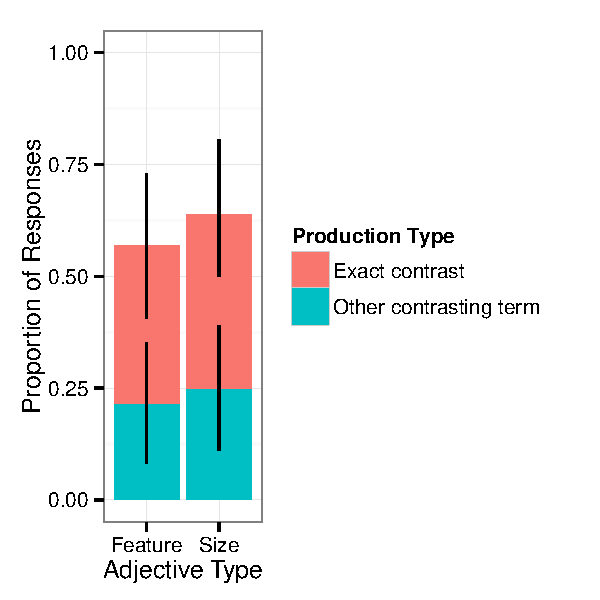
\includegraphics[width=3in]{figures/expt3.pdf} 
    \caption{\label{fig:freeResponse} Four-year-olds' free response descriptions of other category members upon hearing a feature adjective (left) or size adjective (right). Productions were coded as \emph{Exact contrasts} if they were opposite the description and as \emph{Other contrasting terms} if they were related to the target property but neither a direct contrast nor an exact match. Error bars show 95\% confidence intervals. }
  \end{center} 
\vspace{-10ex}
\end{figure}

Despite the open-ended nature of the task, children gave contrastive responses more than half of the time (57\% and 64\% overall for feature and size, Figure \ref{fig:freeResponse}).  We coded responses as either an \emph{Exact contrast} (e.g. hearing ``small'' and saying ``big'') or as an \emph{Other contrasting term} if they were an approximate contrast to the named property (e.g. hearing ``small'' and saying a size property other than ``big'', e.g. ``tall''). Matching, non-contrastive descriptions (e.g. hearing ``small'' and repeating ``small'') were not included in the approximate contrast group. More than a third of productions were exact opposites (35\% for feature terms and 39\% for size terms), and another quarter were non-exact contrasts but related to the stated property information (22\% for feature terms and 25\% for size terms). There were no differences in the proportion of response scores across feature and size trials. Thus, Experiment 5 provides evidence that, even without seeing a contrastive alternative test item, children were able to spontaneously generate appropriate descriptions based on the adjective the speaker used. 

\section{General Discussion}

If a speaker references a ``salad fork,'' can children learn that there are other types of forks? And if they hear someone described as a ``female scientist'' or ``male librarian,'' will they make (potentially harmful) inferences about gender-typical roles? Our findings support the idea that children are indeed sensitive to contrasts of this type. In our experiments, they were able to learn from not just the literal content of a speaker's utterance, but from the choices she made in expressing that content; they inferred property variability from modified noun phrases. Nevertheless, such inferences were not trivial, especially for younger children---a variety of supportive cues to contrast increased performance across studies.

Although the design of our task was simple, it still required children to make a counterintuitive response to the descriptions they heard: inferring that their opposite was typical of a broader category and suppressing a simple perceptual match. This finding is congruent with previous work suggesting that preschoolers make similar inferences in their causal reasoning \cite{harris1996} as well as in their pragmatic use of language \cite{barner2011,stiller2014}. Our task may have been particularly challenging because the paradigm was so contextually minimal, introducing each test trial with a single referential expression. But four-year-olds were still largely able to process the adjective and then select the picture that \emph{differed} from that description instead of the one that shared that property, even though both options were available. Performance was stronger for older children across experiments, however. Because of the inhibitory demands of the task, changes in executive function during the preschool years provide one plausible source for these developmental effects \cite{davidson2006,zelazo2003}. 

Our data speak to children's ability to learn one particular piece of information from pragmatic language use: the typical property for exemplars of a category. We selected this example because the generalization of category structure from individual exemplars is a key problem for children \cite{markman1991}. To test this effect experimentally, we asked children what they thought category members \emph{usually} look like, specifically querying inferences about typicality. But there is a broader variety of inferences that could be made on the basis of the same sort of optional modification. As in the case of ``salad fork,'' sometimes a contrastive modifier does not license specific inferences about what is typical of a category (if ``salad'' does not have an opposite, what can we infer about other forks?). Instead, the modifier licenses the inference that there is some important variability along a dimension (e.g., there are forks for non-salad foods). 

The pragmatic and discourse context of an utterance can also affect the kind of inference that is licensed by a contrastive modifier. Depending on context, labeling someone as a ``good student'' can imply that others in the comparison set are either better (where the student is implied to be ``merely good'') or worse (where the student is ``very good''). Our results suggest that preschoolers are sensitive to property variability conveyed by adjective use, and future work should investigate the broader range of inferences---from other kinds of world knowledge to the idiosyncrasies of social judgement---that are sometimes licensed by adjective use. And in addition to adjectives, many other optional choices that speakers make in their utterances can convey implicit information about the world; consider what is implied about the world by optional modifier phrases like ``a car without a transmission'' (cars usually have transmissions) or ``a politician who thinks that more spending isn't the answer'' (generally, politicians endorse more spending---or at least the speaker thinks this is the case). 

One limitation of our studies here was that all relied on some combination of supportive cues that highlighted the contrastive use of the adjective. All of our studies included contrastive prosody, and several included contrast training or phrases like ``special kind of.'' Children's level of performance in the absence of such cues is an issue for future work, but we speculate that without these supportive cues, four-year-olds would likely not be able to succeed in our task. On the other hand, real-world examples like those given above are likely heard not just once but many times, providing more learning opportunities. Thus, the extent and developmental relevance of learning from purely incidental adjectives remains an open question. 

Our experiments contribute to the growing literature suggesting that children consider how and why evidence is generated to reason about the social world, in both non-linguistic and linguistic contexts. As reviewed above, even young children robustly infer probabilities from random sampling while making inferences about social preferences or generalizable knowledge from conspicuous non-random sampling \cite{xu2009, kushnir2010, butler2012}. In the domain of language, preschoolers are beginning to make similar (pragmatic) inferences about the motivations for language use \cite<e.g.>{stiller2014,katsos2011}, though many factors may constrain their ability to succeed in more complex situations \cite{papafragou2003,barner2011}. 

Most work investigating children's pragmatic abilities has focused on reasoning about speakers' intended meanings. In contrast, we examined children's inferences about the state of the world that would lead a speaker to make particular production choices. While preschoolers show evidence of learning generalizable knowledge from specific descriptions based on framing cues \cite{cimpian2009}, our work suggests an additional pragmatic route to such general knowledge. In this way, we connect the mechanisms of pragmatic inference with processes of social learning and generalization. If children assume that speakers are communicating pragmatically, then they can take advantage of opportunities for learning wherever they recognize a speaker's choice to produce an utterance in one form over another. 


\bibliographystyle{apacite2}
\bibliography{ADJ2}

\newpage
\theappendix 

\section{Appendix A: Materials}

% The full counterbalanced set of materials for Experiment 4 are presented in Table \ref{tab:stimuli}. 

  \begin{table}[h!]
   \caption{: The full counterbalanced set of materials for Experiment 4. 
     \label{tab:stimuli} } 
   \begin{center} 
\resizebox{.9\columnwidth}{!}{
     \begin{tabular}{ccc|c} 
       \hline 
      Induction Example & Contrast 1 & Contrast 2 & Alternative Induction Example\\
       \hline  
\parbox[c]{6.5em}{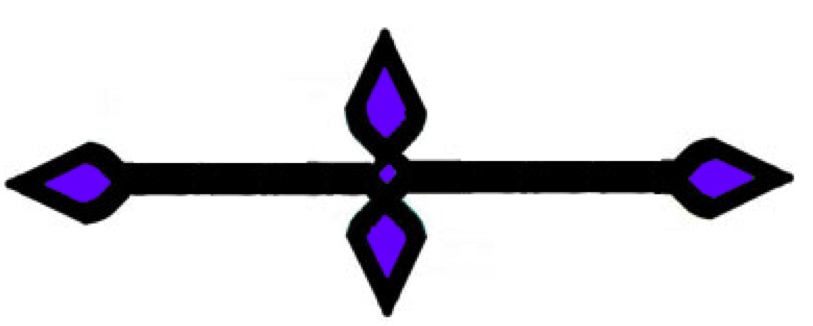
\includegraphics[width=1in]{figures/appendixPix/shape1_a.png}} & \parbox[c]{3em}{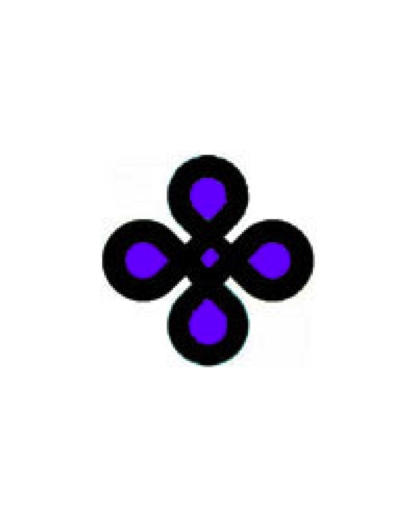
\includegraphics[width=0.5in]{figures/appendixPix/shape1_b.png}} & \parbox[c]{6.5em}{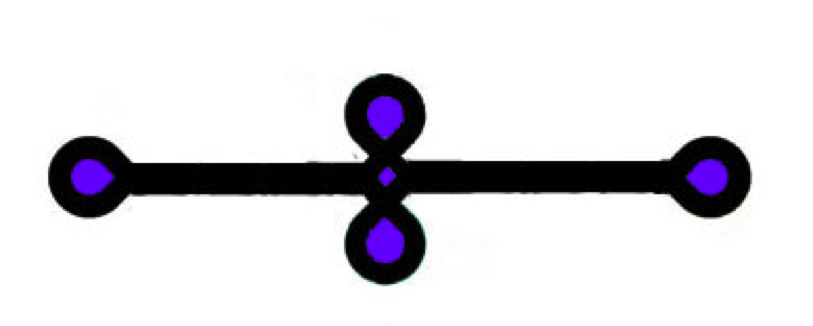
\includegraphics[width=1in]{figures/appendixPix/shape1_c.png}} & \parbox[c]{3em}{
\includegraphics[width=0.5in]{figures/appendixPix/shape1_d.png}}\\
        long / pointy & short / pointy & long / round & short / pointy \\
        \hline
        
        \parbox[c]{6.5em}{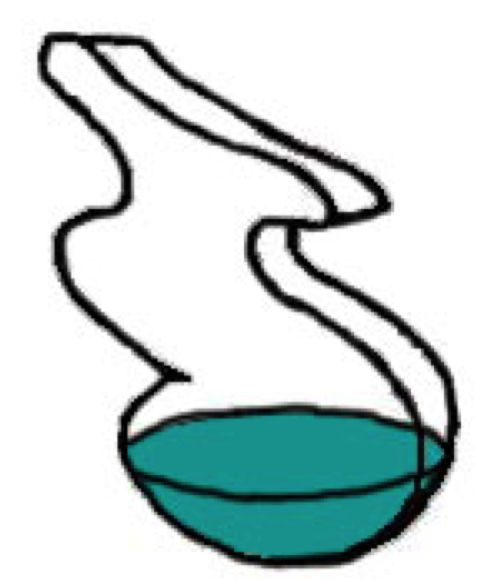
\includegraphics[width=0.7in]{figures/appendixPix/shape2_a.png}} & \parbox[c]{7em}{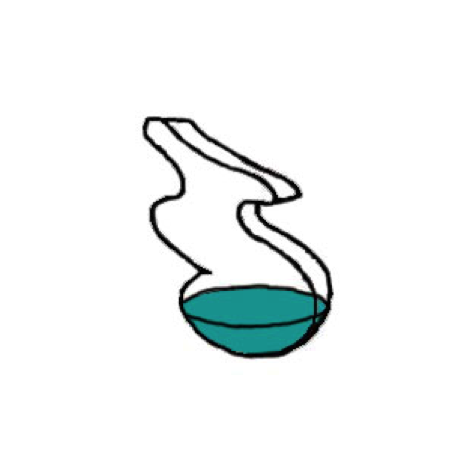
\includegraphics[width=0.85in]{figures/appendixPix/shape2_c.png}} & \parbox[c]{6.5em}{
\includegraphics[width=0.7in]{figures/appendixPix/shape2_b.png}} & \parbox[c]{5em}{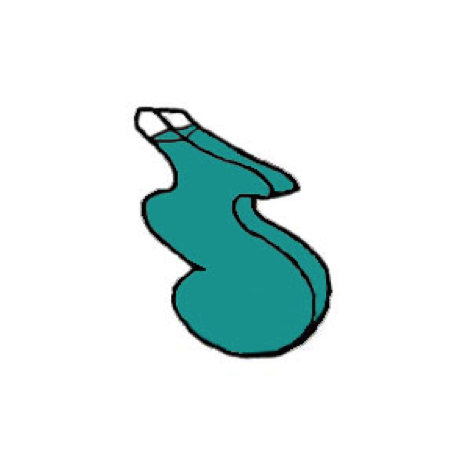
\includegraphics[width=0.8in]{figures/appendixPix/shape2_d.png}}\\
       big / empty   & small / empty & big / full & small / full \\
               \hline 
               
       \parbox[c]{5em}{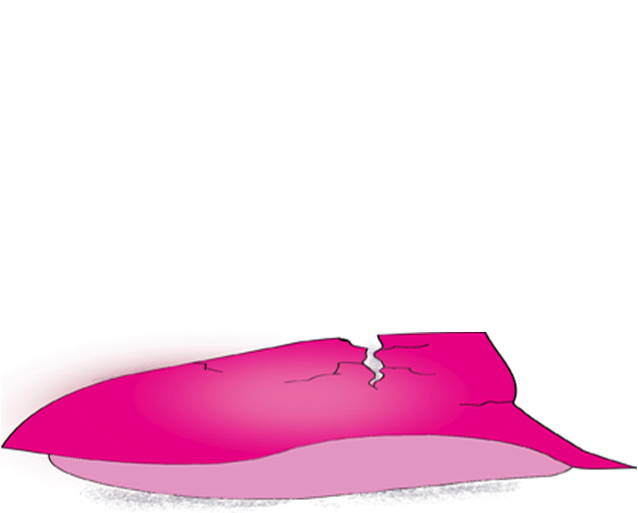
\includegraphics[width=0.7in]{figures/appendixPix/shape3_d.png}} & \parbox[c]{5em}{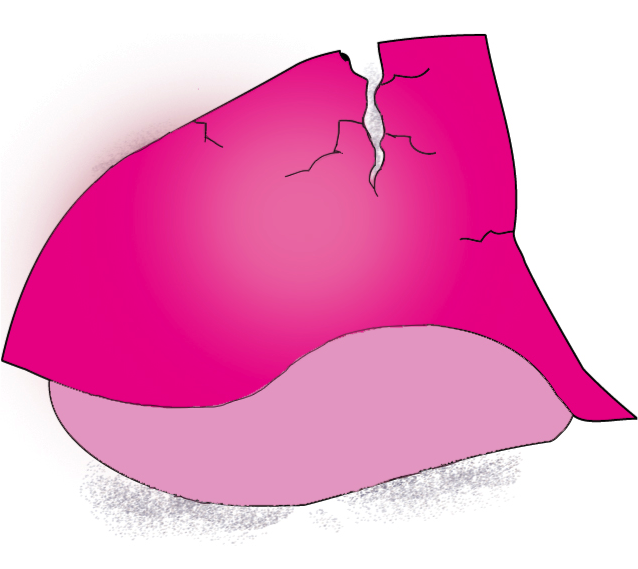
\includegraphics[width=0.7in]{figures/appendixPix/shape3_a.png}} & \parbox[c]{5em}{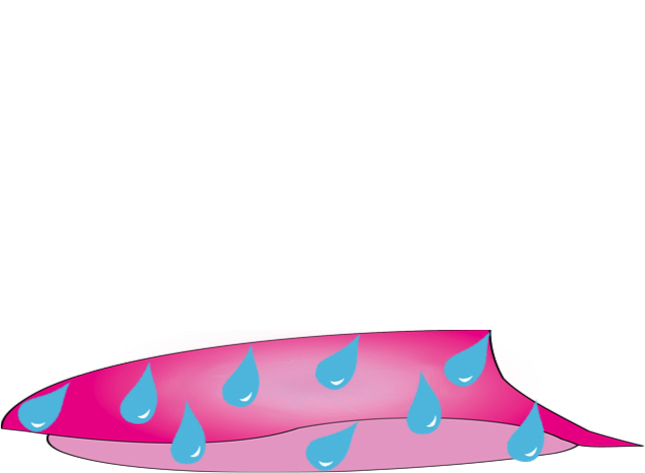
\includegraphics[width=0.7in]{figures/appendixPix/shape3_b.png}} & \parbox[c]{5em}{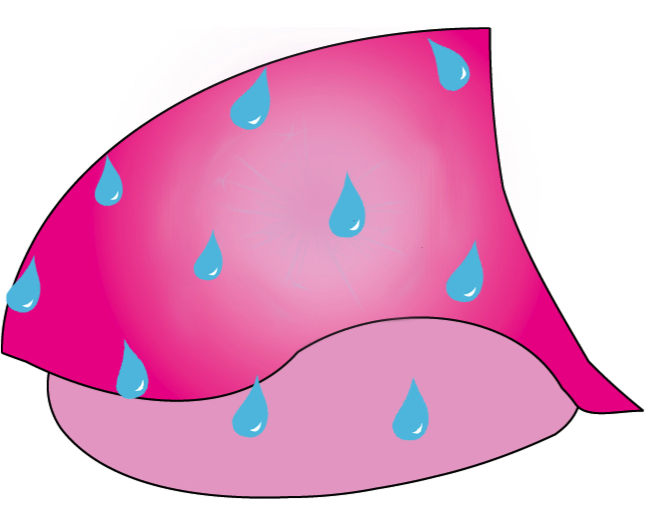
\includegraphics[width=0.7in]{figures/appendixPix/shape3_c.png}}\\
       skinny / dry   & fat / dry & skinny / wet & fat / wet \\
               \hline 
               
               
                      \parbox[c]{3em}{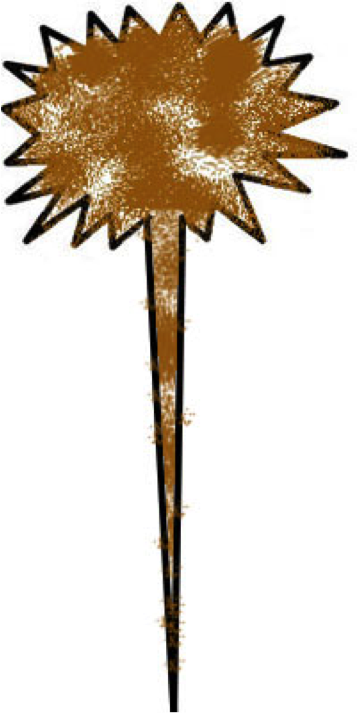
\includegraphics[width=0.48in]{figures/appendixPix/shape8_d.png}} & \parbox[c]{3em}{
\includegraphics[width=0.48in]{figures/appendixPix/shape8_b.png}} & \parbox[c]{3em}{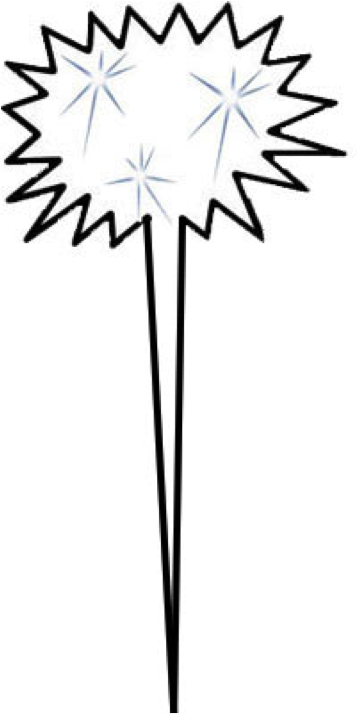
\includegraphics[width=0.5in]{figures/appendixPix/shape8_a.png}} & \parbox[c]{3em}{
\includegraphics[width=0.48in]{figures/appendixPix/shape8_c.png}}\\
       tall / dirty & short / dirty & tall / clean & short / clean \\
               \hline 
               
     \parbox[c]{6em}{
\includegraphics[width=1in]{figures/appendixPix/shape5_d.png}} & \parbox[c]{6em}{
\includegraphics[width=1in]{figures/appendixPix/shape5_a.png}} & \parbox[c]{6em}{
\includegraphics[width=1in]{figures/appendixPix/shape5_b.png}} & \parbox[c]{6em}{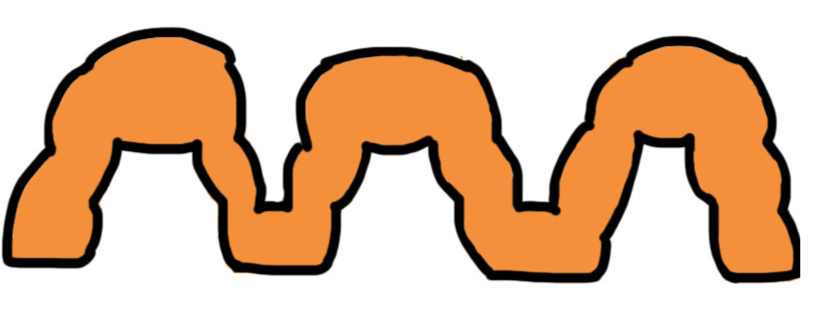
\includegraphics[width=1in]{figures/appendixPix/shape5_c.png}}\\
       short / hard   & long / hard & short / soft & long / soft \\
               \hline 

    \parbox[c]{7em}{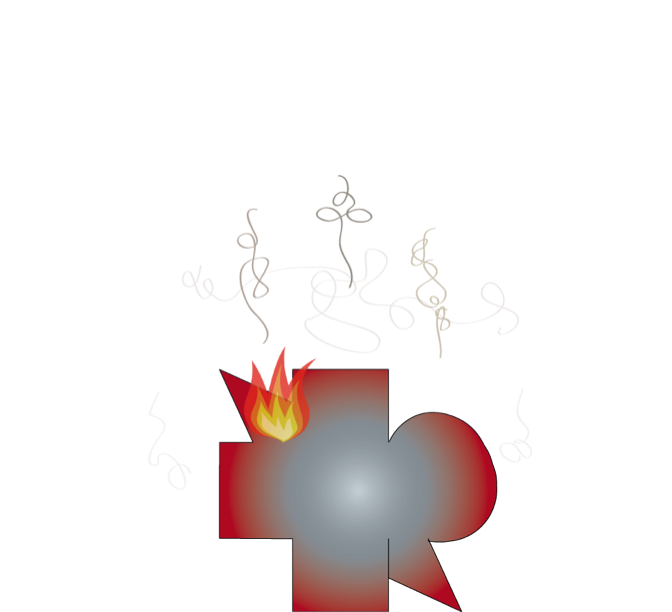
\includegraphics[width=1in]{figures/appendixPix/shape6_b.png}} & \parbox[c]{6em}{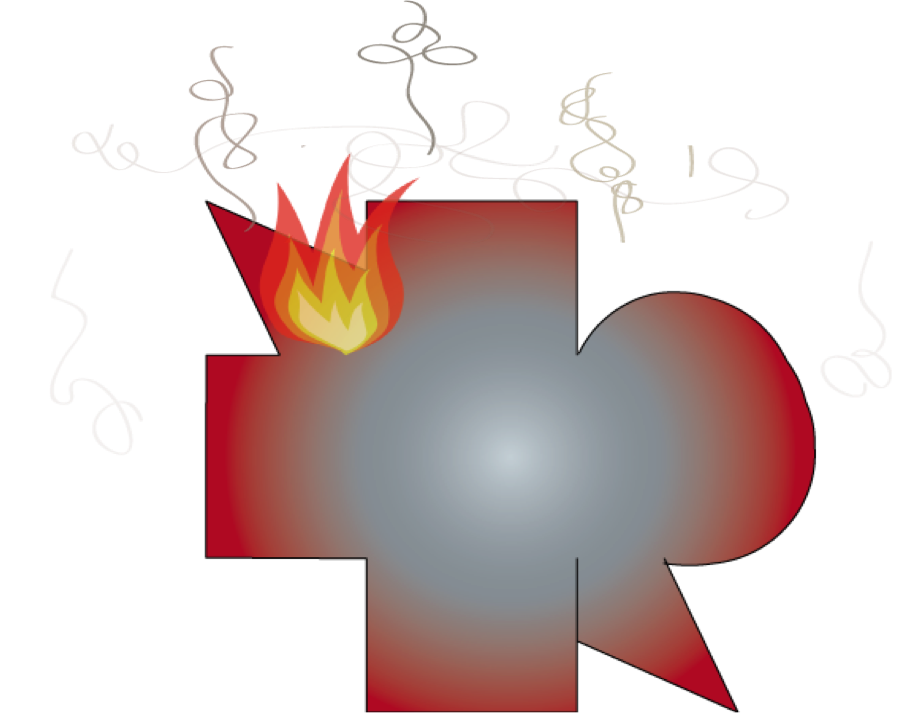
\includegraphics[width=1in]{figures/appendixPix/shape6_d.png}} & \parbox[c]{6em}{
\includegraphics[width=1in]{figures/appendixPix/shape6_c.png}} & \parbox[c]{6em}{
\includegraphics[width=1in]{figures/appendixPix/shape6_a.png}}\\
       small / hot   & big / hot & small / cold & big / cold \\
               \hline 

                   \parbox[c]{5em}{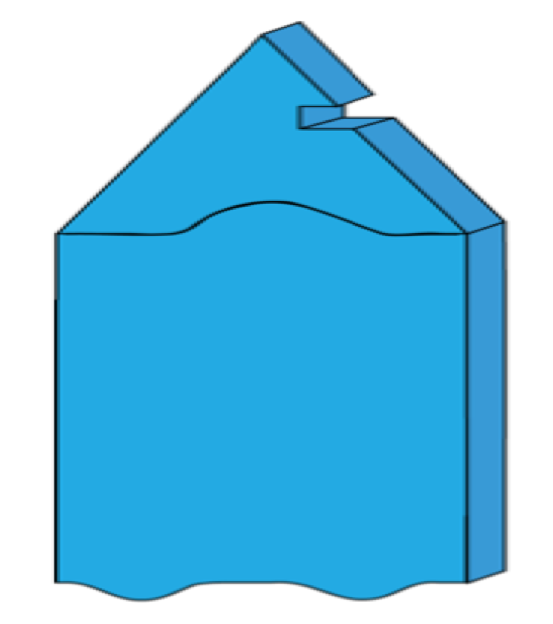
\includegraphics[width=0.7in]{figures/appendixPix/shape7_b.png}} & \parbox[c]{5em}{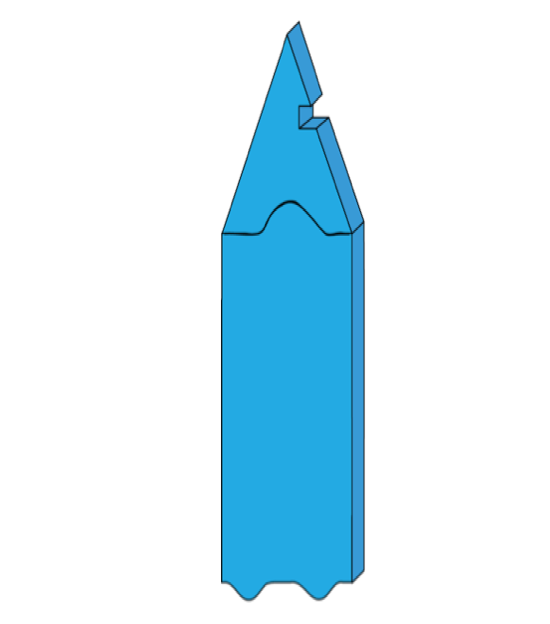
\includegraphics[width=0.7in]{figures/appendixPix/shape7_d.png}} & \parbox[c]{5em}{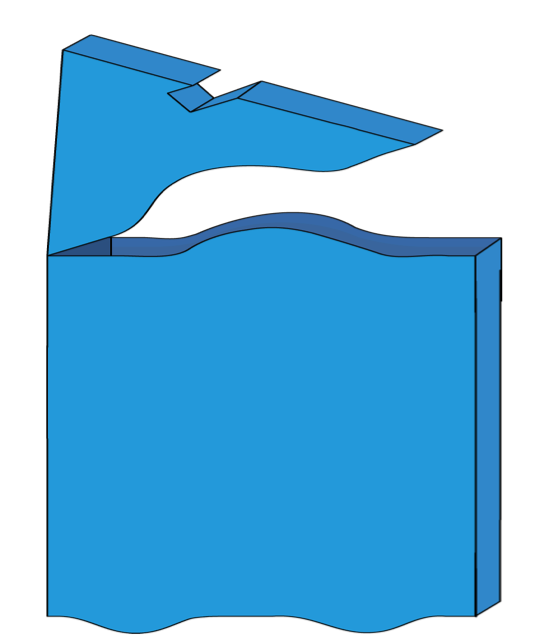
\includegraphics[width=0.7in]{figures/appendixPix/shape7_c.png}} & \parbox[c]{5em}{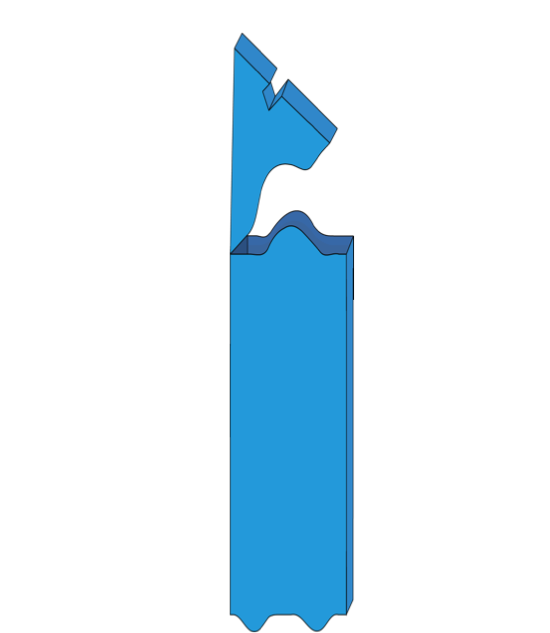
\includegraphics[width=0.7in]{figures/appendixPix/shape7_a.png}}\\
       fat / closed   & skinny / closed & fat / open & skinny / open \\
               \hline 
               
                 \parbox[c]{3em}{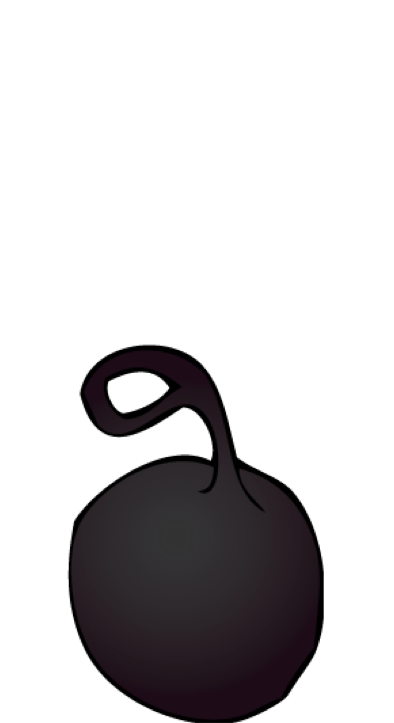
\includegraphics[width=0.4in]{figures/appendixPix/shape4_d.png}} & \parbox[c]{3em}{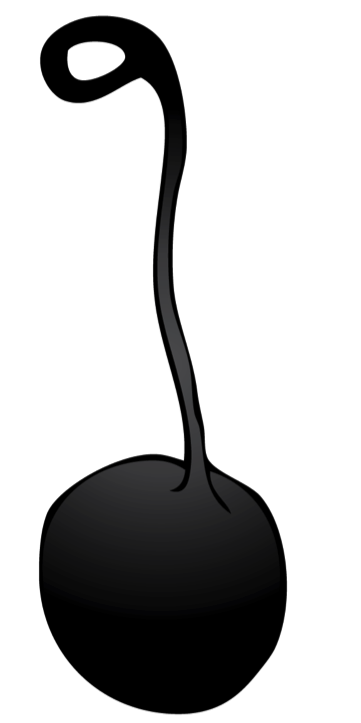
\includegraphics[width=0.4in]{figures/appendixPix/shape4_a.png}} & \parbox[c]{3em}{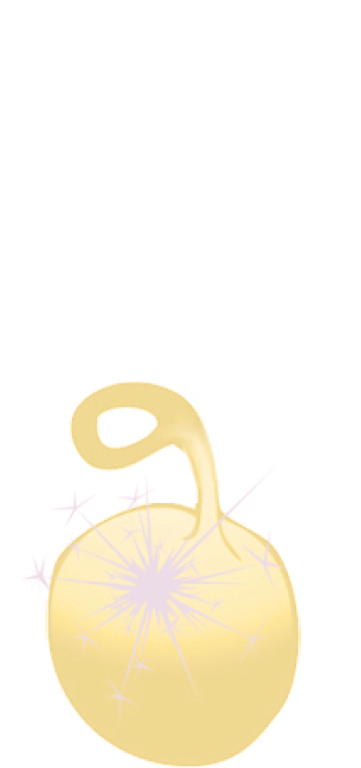
\includegraphics[width=0.4in]{figures/appendixPix/shape4_b.png}} & \parbox[c]{3em}{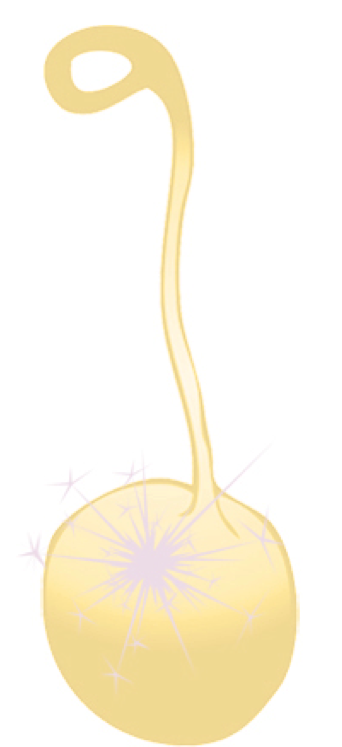
\includegraphics[width=0.4in]{figures/appendixPix/shape4_c.png}}\\
       short / dark   & tall / dark & short / bright & tall / bright \\
               \hline              
     \end{tabular} 
}
  \end{center}
 \end{table}
\end{document}


